\chapter{Coupled Cahn--Hilliard $+$ Allen--Cahn}
\label{ch:p7}

\begin{keybox}
\textbf{Key idea.} The real morphology problem is \emph{coupled}:
composition (Cahn--Hilliard) and crystallinity (Allen--Cahn) evolve
together and feed back. The signature of the coupling is
\emph{crystallization-driven demixing} --- as a species crystallizes it
expels the others, sharpening a composition pattern that phase separation
alone would not produce.
\end{keybox}

\section{The model: the four-fold $\chi$}

With crystallinity, the interaction between two species depends on whether
each is amorphous or crystalline, so the single Flory $\chi$ becomes
\emph{four} matrices:
%
\begin{equation}
  \chi_{\text{eff}}(i,j) = \chi_{aa}
   + \psi_i^2\,\chi_{ca} + \psi_j^2\,\chi_{ac}
   + \psi_i^2\psi_j^2\,\chi_{cc},
   \qquad \chi_{ca}=\chi_{ac}^{\!\top},
\end{equation}
%
coupling the Cahn--Hilliard composition fields to the Allen--Cahn
crystallinity fields. Making $\chi_{ca}$ \emph{larger} than $\chi_{aa}$
means ``a crystal of species $i$ dislikes amorphous species $j$ more than
two amorphous phases dislike each other'' --- so crystallizing $i$ pushes
$j$ out. That is the thermodynamic origin of crystallization-driven
demixing.

\begin{keybox}
\textbf{Coefficients.} The bulk Cahn--Hilliard $\chi_{aa}$ and the
crystal-contact $\chi_{ca}$ (with $\chi_{ca}>\chi_{aa}$ for expulsion),
plus the crystallization energetics of Chapter~\ref{ch:p6} ($\Delta h$,
$\Delta\sigma$, $T$, $T_m$, $\varepsilon^2$, $L_\psi$). The
\emph{demixing metric} is the purity contrast: the mean composition of
the crystallizing species \emph{inside} the crystal ($\psi>0.5$) minus
\emph{outside}.
\end{keybox}

\section{Run it}

\begin{runbox}
\textbf{Run it.}
\begin{lstlisting}
cd physics/07_coupled_ch_ac
python run.py            # crystallization ON vs OFF, then the (M,K) ladder
\end{lstlisting}
It runs $(M,K)=(2,1)$ with crystallization ON and OFF, prints the
demixing purity contrast, and repeats the ON case at $(3,1)$ and $(3,2)$.
Compare with \file{EXPECTED.md} and the figures.
\end{runbox}

\paragraph{What you should see.} With crystallization ON, the
crystallizing species concentrates strongly inside the crystal
(inside $\PsevenInside$ vs outside $\PsevenOutside$; contrast
$\PsevenContrastOn$). With crystallization OFF (the same blend, $K=0$)
the composition only demixes by ordinary Cahn--Hilliard, a much smaller
contrast $\PsevenContrastOff$ --- crystallization amplifies the demixing
by $\PsevenAmplify\times$. The same machinery scales up the ladder:
$(3,1)$ gives contrast $\PsevenContrastThreeone$ and $(3,2)$ gives
$\PsevenContrastThreetwo$.

% --- generated by gen_figures.py ---
\begin{figure}[h]\centering
  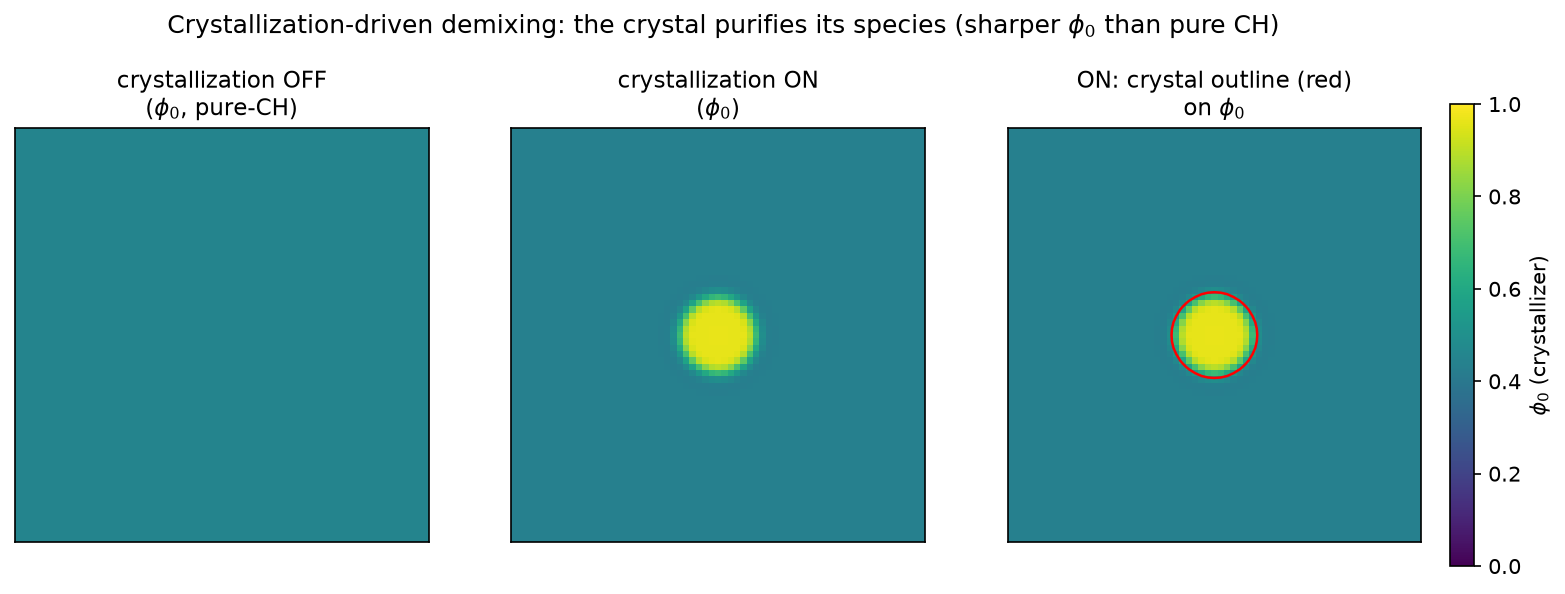
\includegraphics[width=\linewidth]{figures/p7_demixing.png}
  \caption{Crystallization-driven demixing at $(M,K)=(2,1)$. Left:
    crystallization off (pure Cahn--Hilliard composition). Middle/right:
    crystallization on --- the crystal (red outline) purifies its species,
    a sharper composition pattern than phase separation alone produces.}
  \label{fig:p7demix}
\end{figure}

\begin{figure}[h]\centering
  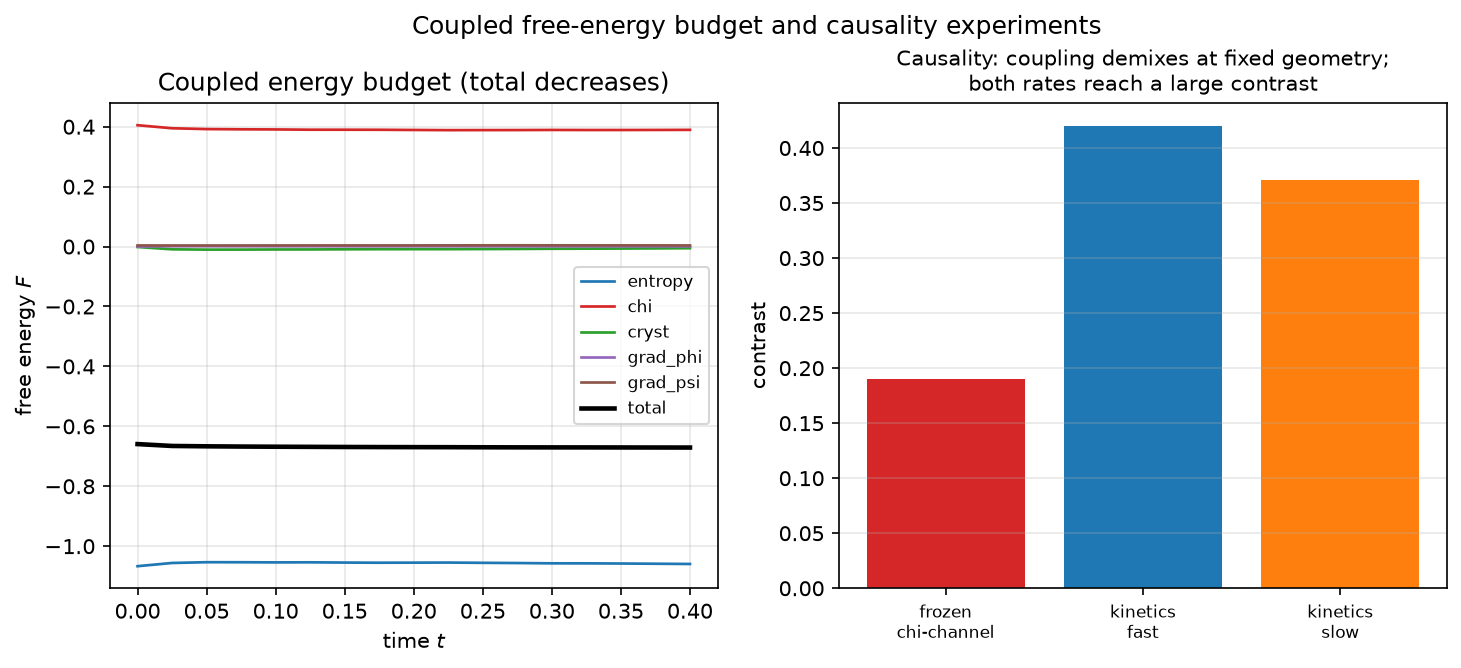
\includegraphics[width=\linewidth]{figures/p7_ladder.png}
  \caption{The same coupled model up the $(M,K)$ ladder:
    $(2,1)\to(3,1)\to(3,2)$. Adding species and crystallizable phases is
    a change of two integers; the physics (crystallization-driven
    demixing) carries over.}
  \label{fig:p7ladder}
\end{figure}

\begin{keybox}
\textbf{Measured self-check.}
\begin{center}\small
\begin{tabular}{lc}
\toprule
$(2,1)$ crystallizer $\phi_0$: inside $\to$ outside crystal & $\PsevenInside \to \PsevenOutside$ \\
demixing contrast: ON vs OFF & $\PsevenContrastOn$ vs $\PsevenContrastOff$ \\
amplification (ON/OFF) & $\PsevenAmplify\times$ \\
contrast at $(3,1)$ / $(3,2)$ & $\PsevenContrastThreeone$ / $\PsevenContrastThreetwo$ \\
\bottomrule
\end{tabular}
\end{center}
\end{keybox}

\section{Code walk-through}

\paragraph{1. Four $\chi$ matrices.} \code{\_chis} builds the amorphous
$\chi_{aa}$ (all pairs) and the stronger crystal-contact $\chi_{ca}$
(a crystallizing species vs the others); passing them to
\code{MultiPhaseStepper(chi\_aa=..., chi\_ac=..., chi\_ca=...)} turns on
the coupling.

\paragraph{2. ON vs OFF control.} The same call with $K=0$ drops the
crystal terms, isolating the pure-Cahn--Hilliard demixing --- the control
that makes the crystallization contribution measurable.

\paragraph{3. The purity contrast.} The demixing metric splits the field
by the crystal mask $\psi>0.5$ and differences the mean composition,
inside vs outside.

\section{Explore on your own}

\question{Sweep $\chi_{ca}$ from $\chi_{aa}$ (no extra crystal repulsion)
upward. At what point does crystallization-driven demixing switch on, and
how does the purity contrast scale with $\chi_{ca}-\chi_{aa}$?}

\question{Turn crystallization on \emph{after} the blend has partly
demixed (delay the seed). Does the crystal template on the existing
composition pattern, or reshape it? What does this say about processing
order (phase-separate then crystallize vs simultaneously)?}

\question{At $(3,2)$ two species crystallize. Do their crystals compete
for the same regions, or segregate? How does the second crystallizable
phase change the amorphous matrix left behind?}

\question{Compare the coarsening rate with and without crystallization.
Does the growing crystal \emph{pin} the composition pattern (slower
coarsening), and why would a device designer want that?}

\question{The contrast is a purity measure. Relate it to what a solar
cell wants (pure domains for transport, but a bicontinuous network for
charge separation). Is more contrast always better?}

% ====================================================================
